\begin{frame}{Trigger software profiling}
\begin{columns}[c]
\column{.4\textwidth}
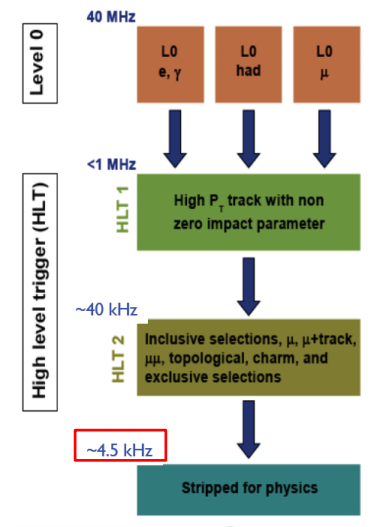
\includegraphics[width=.9\textwidth]{profiler/hlt_struct1.png}\\~\\
\textcolor{red}{The trigger needs fast algorithms!}
\column{.6\textwidth}
Most experiments require a trigger in order to record interesting events at suitable rate.
\begin{itemize}
  \item L0 Hardware Trigger $40 MHz \rightarrow 1 MHz$. Search for high pt, $\mu$, e, $\gamma$, hadron candidates.
  \item High Level Software Trigger Farm
  \begin{itemize}
    \item HLT1: Add Impact parameter cuts
    \item HLT2: Global event reconstruction.
  \end{itemize}
\end{itemize}
\begin{itemize}
  \item 100 man/years work that has only 20-30 ms to process an average event.
  \item 29K CPUs or 1700 servers.
  \item $2 \times 10^{15}$ bytes stored in 2012.
\end{itemize}
% \includegraphics[width=.8\textwidth]{images/moore.png}
\end{columns}
\end{frame}
